\documentclass{article}
\usepackage{lucidabr,amsmath}
\usepackage{verbatim,fancyvrb}
\usepackage{color,mycode}
\usepackage{graphicx}
\usepackage{smallhds,url}
\usepackage{hyperref}

\usepackage[letterpaper,body={6.3in,9.15in},top=.8in,left=1.1in]{geometry}
% \usepackage[a4paper,body={6.1in,9.7in},top=.8in,left=1.1in]{geometry}

\hypersetup{pdftitle={random_forest 0.1},
            pdfauthor={Allin Cottrell},
            colorlinks=true,
            linkcolor=blue,
            urlcolor=red,
            citecolor=steel,
            bookmarks=true,
            bookmarksnumbered=true,
            plainpages=false
}

\begin{document}

\setlength{\parindent}{0pt}
\setlength{\parskip}{1ex}

\title{random\_forest 0.1} \author{Allin Cottrell}
\maketitle

This is an unusual gretl package---unusual (but not illegal!) in that
it relies on the \textsf{R} package \textsf{randomForest} for its
underlying functionality,\footnote{See
  \url{https://cran.r-project.org/web/packages/randomForest/index.html}.}
and therefore also relies on \textsf{R} itself. A native
implementation of the Random Forest machine-learning algorithm may be
added to gretl at some point, but for now the aim of this package is
more modest: simply to offer a gretl-style scripting interface, as
well as a gretl-style GUI interface, to functionality borrowed from
the \textsf{R} ecosystem.

This package was last verified as working with \textsf{R} version
4.2.1 (2022-06-23) and \textsf{randomForest} 4.7-1.1 (2022-05-23),
which requires \textsf{R} 4.1.0 or higher. Some details about ensuring
the \textsf{R} setup that's required can be found in the Appendix to
this document.

I'm not going to try explaining here what the Random Forest algorithm
is all about---I think Wikipedia does a good job,\footnote{See
  \url{https://en.wikipedia.org/wiki/Random_forest}.} and you can
consult Leo Breiman's original paper on the topic.\footnote{See
  \url{https://www.stat.berkeley.edu/~breiman/randomforest2001.pdf}.}
I'll just say that it's a predictive apparatus somewhat comparable
with a Support Vector Machine or SVM, something that is supported
natively in gretl---see ``gretl + SVM'' under the \textsf{Help} menu
in the gretl GUI.

\section{Scripting usage}

The function available for command-line and scripting use is named
\texttt{random\_forest}. It has the following signature:
%
\begin{code}
bundle random_forest (list L, const bundle opts)
\end{code}
%
This means that it returns a bundle and has two required arguments, a
list and a bundle. The list argument should be in standard gretl
``regression list'' format: the dependent variable followed by one or
more independent variables (or ``features'' as they're known in the
machine-learning world). The \texttt{opts} bundle has just one
required member: under the key \texttt{n\_train} you must tell gretl
how many of the available observations should be used for training.
The remaining observations (there must be some left over) will be used
for testing. What you get on return is a bundle containing predictions
for both the training and the testing data, along with some figures of
merit with which to assess the degree of predictive success.

We'll expand on the content of the bundle returned by
\texttt{random\_forest} shortly. First of all here's some detail on
the options. Besides \texttt{n\_train}, the \texttt{opts} bundle may
contain any of the following:

\begin{center}
\begin{tabular}{llll}
  \textit{key} & \textit{type} & \textit{comment} & \textit{default value} \\[4pt]
  \texttt{verbose} & integer & controls printed output & 1 \\
  \texttt{classify} & boolean & classification (vs. regression) & automatic\\
  \texttt{tune} & boolean & tune the \texttt{mtry} parameter & 1 or TRUE \\
  \texttt{seed} & integer & seed for RNG in \textsf{R} & automatic
\end{tabular}
\end{center}

The default \texttt{verbose} value of 1 prints summary output compiled
by gretl. The other acceptable values are 0, for no printed output, or
2, to include a trace of the progress made by \textsf{R}'s
\textsf{randomForest}.

The Random Forest algorithm can handle both ``classification'' (for
discrete, qualitative outcomes) and ``regression'' (for a more or less
continuous numerical outcome). By default gretl will call for
classification if and only if the dependent variable is a 0/1 dummy
variable or is marked as an ``encoding'' (see the help for the
\texttt{setinfo} command).  But you can force the issue by setting
\texttt{classify} to 0 or 1. (You may wish to take control when the
dependent is ordinal, but not on an interval or ratio scale.)

Unless you're in a big hurry you'll likely want to let the underlying
engine do some tuning. This involves a call to the \texttt{tuneRF}
function in the \textsf{R} package. The tunable parameter
\texttt{mtry} represents the number of covariates randomly sampled as
candidates at each split in tree formation; \texttt{tuneRF} optimizes
this parameter with respect to an ``Out-of-Bag'' error estimate.  If
you just want to use the default value of \texttt{mtry}, give
\texttt{0} or \texttt{FALSE} for the \texttt{tune} option. In
classification mode the default is $\sqrt{k}$ and in regression mode
it's $k/3$, where $k$ is the number of covariates.

As the name implies, there's randomization involved in building a
Random Forest. If you want to get perfectly reproducible results you
should set \texttt{seed} to a specific value in the options bundle;
otherwise the results will differ to some degree across runs of a
given script.

We'll illustrate a call to \texttt{random\_forest} by reference to the
sample script included in the package.  It begins with
%
\begin{code}
include random_forest.gfn
open titanic3.gdt -q --frompkg=random_forest
set seed 877777
series sorter = uniform()
dataset sortby sorter
\end{code}
%
The data file is a slightly modified version of \texttt{titanic3.csv}
from \url{https://hbiostat.org/data/}; it contains 1306 records
regarding passengers on RMS \textit{Titanic}.\footnote{A subset of
  these data can be found at \url{https://www.kaggle.com/c/titanic}.}
The target for prediction is the binary variable \texttt{survived} (1
= survived, 0 = didn't). Seven other variables are available as
candidate predictors.  The last two lines of the extract above
randomize the order of the observations prior to division into
training and testing samples.  (You can comment out the \texttt{set
  seed} statement to get a different randomization on each invocation
of the script).  The code then continues:
%
\begin{code}
list L = survived pclass female sibsp parch fare embarked
bundle opts = _(n_train=900, seed=777778)
bundle rfb = random_forest(L, opts)
\end{code}
%
So we're using six of the covariates,\footnote{The \texttt{age}
  variable is potentially useful but is missing in 263 cases so we
  omitted it here.}  selecting the first 900 records for training,
setting a random seed for replicability (this seed will be used by
\textsf{R}), and implicitly accepting the default values for
classification mode, \texttt{tune} and \texttt{verbose}.

Partial output from the sample script is shown in
Listing~\ref{output}.

\begin{script}[htbp]
  \begin{scodebit}
Called randomForest() in classification mode
Dependent variable: survived
Total observations 1306: 900 training, 406 testing
RNG seed = 777778

Training percent correct: 78.33
Testing percent correct:  80.30

Confusion matrix, training:
             0            1

0          473           71
1          124          232

Confusion matrix, testing:
             0            1

0          226           38
1           42          100
\end{scodebit}
  \caption{Output from sample script}
  \label{output}
\end{script}

\subsection{The returned bundle}

The bundle returned by \texttt{random\_forest} in classification mode
contains the following items.
\begin{itemize}
\item Column vectors named \texttt{insample} and \texttt{outsample}
  holding the predictions for the training and testing observations,
  respectively. Plus, for convenience, a vector named \texttt{allpred}
  holding all the predictions. These vectors can easily be converted
  into series if needed.
\item Scalars \texttt{pcc1} and \texttt{pcc2} giving the percentage of
  correct predictions for the training and testing data respectively.
\item Confusion matrices \texttt{C1} and \texttt{C1} pertaining to the
  training and testing data.
\end{itemize}

In case the mode is regression rather than classification, the
\texttt{insample}, \texttt{outsample} and \texttt{allpred} values are
as described above, but \texttt{pcc1} and \texttt{pcc2} are replaced
by \texttt{MSE1} and \texttt{MSE2}, giving the mean squared error for
the two sub-samples, and \texttt{C1} and \texttt{C1} are replaced by a
single matrix named \texttt{regstats}, an example of which is shown
below.
%
\begin{code}
         Training      Testing 
  ME       453.91      -8666.1 
RMSE       44776.       51341. 
 MAE       29757.       36842. 
 MPE      -5.2256      -13.368 
MAPE       15.756       22.104
\end{code}
%
The abbreviated row labels in \texttt{regstats} expand as follows:
\texttt{ME} = mean error, \texttt{RMSE} = root mean squared error,
\texttt{MAE} = mean absolute error, \texttt{MPE} = mean perecentage
error, and \texttt{MAPE} = mean absolute percentage error.


\section{GUI usage}

On installing the package you should be given the option of adding a
hook named \textsf{Random Forest} to gretl's \textsf{Model} menu, under
the \textsf{Robust estimation} sub-menu. This hook brings up a
dialog box in which you can select the various inputs described above
(Figure~\ref{fig:dialog}). Clicking \textsf{OK} in this dialog will
open a window displaying the results of estimation and allowing you to
save the results bundle and/or any of its contents.

\begin{figure}[htbp]
  \centering
  %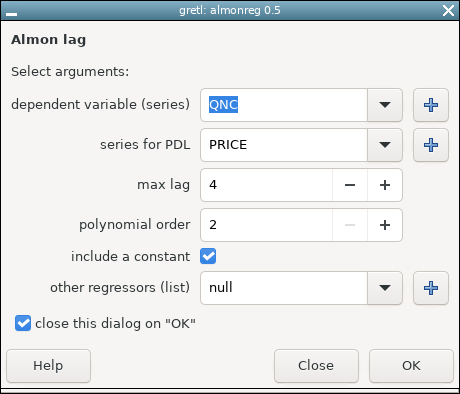
\includegraphics[scale=0.6]{almonreg.png}
  \caption{The random\_forest dialog}
  \label{fig:dialog}
\end{figure}

\section*{Change log}

2023-02-05: version 0.1 released.

\section*{Appendix}

To be written.

\end{document}
